% =====================================================================
%  MCMP117 -- Fundamentals of Operating Systems
%  Week 3 Course Notes: OS Services, System Calls & Processes
%  Compile with XeLaTeX (twice):  xelatex MCMP117_Week3_Notes.tex
%  Needs ./figures/ and the ../code/ folder.
% =====================================================================
\documentclass[11pt,a4paper]{article}
\newcommand{\weeknum}{3}
% ---------- Page & fonts ---------------------------------------------
\usepackage[a4paper,margin=2.3cm,headheight=15pt]{geometry}
\usepackage{fontspec}
\IfFontExistsTF{Calibri}{\setmainfont{Calibri}}{\setmainfont{Carlito}}
\IfFontExistsTF{Cambria}{\newfontfamily\headfont{Cambria}}{\newfontfamily\headfont{Caladea}}
\IfFontExistsTF{Consolas}{\setmonofont[Scale=0.95]{Consolas}}{\setmonofont[Scale=0.88]{DejaVu Sans Mono}}
\usepackage{amsmath,amssymb}
\usepackage{microtype}
\linespread{1.12}
\setlength{\parskip}{0.55em}
\setlength{\parindent}{0pt}

% ---------- Colours (course design system) ----------------------------
\usepackage{xcolor}
\definecolor{dark}{HTML}{212121}
\definecolor{charcoal}{HTML}{36454F}
\definecolor{slate}{HTML}{50808E}
\definecolor{mint}{HTML}{02C39A}
\definecolor{mintdeep}{HTML}{028090}
\definecolor{light}{HTML}{F2F2F2}
\definecolor{muted}{HTML}{6B7679}

% ---------- Packages ---------------------------------------------------
\usepackage{graphicx}
\usepackage{float}
\usepackage{needspace}
\graphicspath{{figures/}}
\usepackage[font=small,labelfont={bf,color=mintdeep},justification=centering]{caption}
\usepackage{booktabs,longtable,array,tabularx}
\usepackage{enumitem}
\setlist{itemsep=0.25em,topsep=0.3em}
\usepackage{tikz}
\usetikzlibrary{arrows.meta,positioning,calc,shapes.geometric}
\usepackage{pgfplots}
\pgfplotsset{compat=1.17}
\usepackage[most]{tcolorbox}
\usepackage{titlesec}
\usepackage{fancyhdr}
\usepackage{xurl}
\usepackage[colorlinks=true,linkcolor=mintdeep,urlcolor=mintdeep,citecolor=mintdeep]{hyperref}

% ---------- Headings ----------------------------------------------------
\titleformat{\section}{\headfont\Large\bfseries\color{charcoal}}{\color{mint}\thesection}{0.7em}{}
\titleformat{\subsection}{\headfont\large\bfseries\color{charcoal}}{\color{mintdeep}\thesubsection}{0.6em}{}
\titleformat{\subsubsection}{\headfont\normalsize\bfseries\color{mintdeep}}{}{0em}{}
\titlespacing*{\section}{0pt}{1.6em}{0.6em}
\titlespacing*{\subsection}{0pt}{1.2em}{0.4em}

% ---------- Header / footer -----------------------------------------------
\pagestyle{fancy}
\fancyhf{}
\fancyhead[L]{\small\color{muted}MCMP117 --- Fundamentals of Operating Systems}
\fancyhead[R]{\small\color{muted}Week \weeknum{} Notes}
\fancyfoot[C]{\small\color{muted}\thepage}
\renewcommand{\headrulewidth}{0pt}

% ---------- Boxes ---------------------------------------------------------
\newtcolorbox{keyidea}[1][Key idea]{enhanced,breakable,colback=charcoal,colframe=charcoal,
  coltext=white,fonttitle=\headfont\bfseries\color{mint},title={#1},
  attach title to upper={\par\smallskip},boxrule=0pt,arc=3pt,left=10pt,right=10pt,top=8pt,bottom=8pt}
\newtcolorbox{example}[1][Worked example]{enhanced,colback=light,colframe=light,
  fonttitle=\headfont\bfseries\color{mintdeep},title={#1},attach title to upper={\par\smallskip},
  boxrule=0pt,arc=3pt,left=10pt,right=10pt,top=8pt,bottom=8pt}
\newtcolorbox{tryit}[1][Try it yourself]{enhanced,breakable,colback=white,colframe=mint,
  fonttitle=\headfont\bfseries\color{mintdeep},title={#1},attach title to upper={\par\smallskip},
  boxrule=0.8pt,arc=3pt,left=10pt,right=10pt,top=8pt,bottom=8pt}
\newtcolorbox{histnote}[1][Historical note]{enhanced,breakable,colback=white,colframe=slate!40,
  fonttitle=\headfont\bfseries\color{slate},title={#1},attach title to upper={\par\smallskip},
  boxrule=0.5pt,arc=3pt,left=10pt,right=10pt,top=8pt,bottom=8pt,fontupper=\small}

% Photo helper: fits image inside a box, never distorted (keepaspectratio)
\newcommand{\photo}[3]{\includegraphics[width=#1,height=#2,keepaspectratio]{#3}}

\newcommand{\term}[1]{\textbf{\color{mintdeep}#1}}
\newcommand{\cmd}[1]{\texttt{#1}}


% ---------- Code listings ----------------------------------------------------
\usepackage{listings}
\lstdefinestyle{course}{
  basicstyle=\ttfamily\small, columns=fullflexible, keepspaces=true,
  backgroundcolor=\color{dark}, rulecolor=\color{dark}, frame=single, framesep=6pt,
  xleftmargin=8pt, xrightmargin=8pt, aboveskip=0.8em, belowskip=0.6em,
  basicstyle=\ttfamily\small\color{light},
  keywordstyle=\color{mint}\bfseries, commentstyle=\color{white!60}\itshape,
  stringstyle=\color{orange!70!yellow}, numberstyle=\tiny\color{muted},
  numbers=left, numbersep=10pt, showstringspaces=false, breaklines=true,
  tabsize=4, upquote=true}
\lstdefinestyle{term}{style=course, numbers=none, keywordstyle=\color{light},
  commentstyle=\color{white!60}, stringstyle=\color{light}}
\lstset{style=course,language=C}
\usepackage{textcomp}

\begin{document}
% ============================ Week 3 body ============================
\setlength{\emergencystretch}{3em}
\tcbset{breakable}
\lstset{style=course,language=C,basicstyle=\ttfamily\footnotesize\color{light}}
\thispagestyle{empty}
\begin{tcolorbox}[enhanced,colback=dark,colframe=dark,arc=0pt,boxrule=0pt,
  left=18pt,right=18pt,top=20pt,bottom=20pt,coltext=white]
{\small\color{mint}\textsc{MCMP117 \,·\, Week 3 \,·\, Course Notes}}\par\medskip
{\headfont\fontsize{26}{30}\selectfont\bfseries Fundamentals of Operating Systems}\par\medskip
{\large Operating-System Services, System Calls \& Processes}\par\smallskip
{\small\itshape\color{white!70} What does the OS do for a program --- and what exactly is a running program?}
\end{tcolorbox}

\vspace{0.4em}
{\small
\textbf{Instructor:} Asst.\ Prof.\ Dr.\ (Ph.D.) Hasan Oğuz\\
Head of the Electronical Communication Technology Programme, Vocational School\\
Istanbul Okan University\par}

\vspace{0.8em}
\begin{keyidea}[What you should be able to do after this week]
\begin{enumerate}[leftmargin=1.4em]
  \item List the services an operating system provides to users and programs, and the services it needs for its own efficient operation.
  \item Distinguish an API function, a library wrapper and a system call, and trace one \cmd{write()} from a C program into the kernel and back.
  \item Explain the system-call table, the three ways of passing parameters, and the six categories of system calls.
  \item Explain the difference between a program and a process and draw the memory layout of a process (text, data, bss, heap, stack).
  \item Draw the five-state process diagram, say what triggers each transition, and list the contents of a process control block (PCB).
  \item Describe a context switch and compute its overhead; explain \cmd{fork()}, \cmd{exec()} and \cmd{wait()}, zombies and orphans, and count the processes created by a loop of \cmd{fork()} calls.
\end{enumerate}
\end{keyidea}

\setcounter{tocdepth}{1}
\tableofcontents

% =====================================================================
\section*{Where we left off}
In Week~2 we met \term{dual-mode operation} and watched a first \term{system call} with \cmd{strace}: \cmd{printf()} ended up as \cmd{write(1, \dots)}, and a minimal system call cost about $116$~ns, roughly $76$ times a function call. This week we ask which services sit behind the system-call door (Section~\ref{sec:services}) and how a request travels through it (Section~\ref{sec:syscalls}); then we turn to the \term{process} (Sections~\ref{sec:process}--\ref{sec:creation}).

% =====================================================================
\section{Operating-System Services}
\label{sec:services}

An operating system provides an environment in which programs run. The specific services differ from one OS to another, but the common ones fall into two groups: services that help the \emph{user} (and the user's programs), and services that keep the \emph{system itself} running efficiently and safely when many users and programs share it.

\begin{figure}[H]
\centering
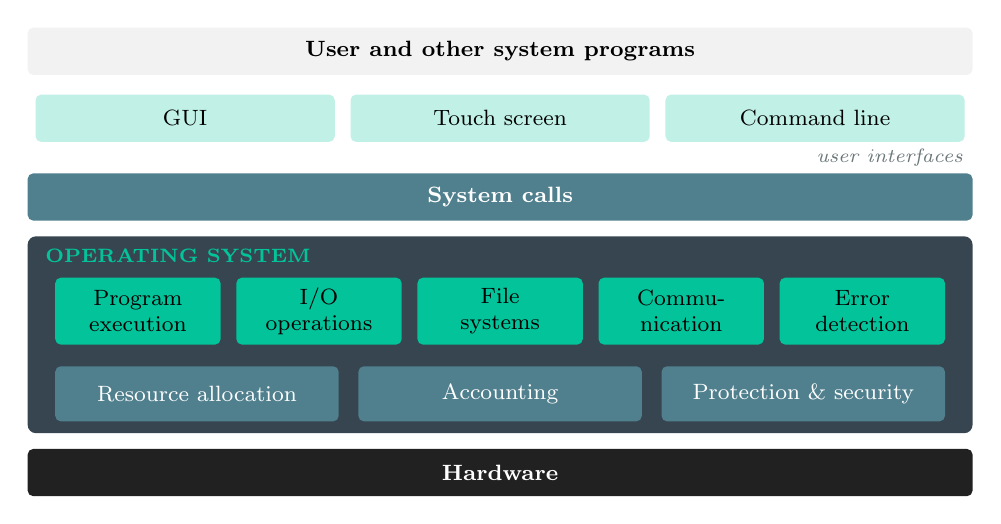
\begin{tikzpicture}[
  b/.style={rectangle,rounded corners=2pt,minimum height=0.6cm,align=center,font=\footnotesize},
  wide/.style={b,minimum width=12cm}]
\node[wide,fill=light] at (0,3.6) {\textbf{User and other system programs}};
\foreach \x/\t in {-4/GUI, 0/Touch screen, 4/Command line} \node[b,fill=mint!25,minimum width=3.8cm] at (\x,2.75) {\t};
\node[font=\scriptsize\itshape,text=muted,anchor=east] at (6,2.25) {user interfaces};
\node[wide,fill=slate,text=white] at (0,1.75) {\textbf{System calls}};
\fill[charcoal,rounded corners=3pt] (-6,-1.25) rectangle (6,1.25);
\node[font=\scriptsize\bfseries,text=mint,anchor=west] at (-5.9,1.0) {OPERATING SYSTEM};
\foreach \i/\t in {0/{Program\\execution},1/{I/O\\operations},2/{File\\systems},3/{Commu-\\nication},4/{Error\\detection}}
  \node[b,fill=mint,minimum width=2.1cm,minimum height=0.85cm] at (-4.6+\i*2.3,0.3) {\t};
\foreach \i/\t in {0/{Resource allocation},1/{Accounting},2/{Protection \& security}}
  \node[b,fill=slate,text=white,minimum width=3.6cm,minimum height=0.7cm] at (-3.85+\i*3.85,-0.75) {\t};
\node[wide,fill=dark,text=white] at (0,-1.75) {\textbf{Hardware}};
\end{tikzpicture}
\caption{A view of operating-system services (after Silberschatz et al., Fig.~2.1). Mint: services for the user; slate: services for the system itself.}
\end{figure}

\subsection{Services that help the user}

\begin{itemize}
  \item \textbf{User interface.} Almost every OS has one. A \term{command-line interface} (CLI) reads typed commands; a \term{graphical user interface} (GUI) uses windows, icons and a pointer; phones and tablets use a \emph{touch-screen} interface; and a \emph{batch} interface reads commands from a file.
  \item \textbf{Program execution.} The OS loads a program into memory, runs it, and ends it, either normally or abnormally (with an error code).
  \item \textbf{I/O operations.} A running program may need a file or a device. Because of dual mode, programs cannot drive devices themselves; the OS performs the I/O for them.
  \item \textbf{File-system manipulation.} Programs create, delete, read, write and search files and directories, and manage their permissions.
  \item \textbf{Communication.} Processes exchange information, either on the same computer or between computers over a network. This is done with \term{shared memory} (two processes read and write the same memory area) or with \term{message passing} (the OS moves packets of data between processes, e.g.\ pipes and sockets).
  \item \textbf{Error detection.} Errors can happen in the CPU and memory, in devices (a disk read fails, a network link goes down, the printer runs out of paper) and in user programs (division by zero, an access to a forbidden address). For each type of error the OS must take the right action: retry, report, or terminate the program.
\end{itemize}

\subsection{Services for the system itself}

\begin{itemize}
  \item \textbf{Resource allocation.} When several users or jobs run at the same time, each must get its share of the CPU, memory, files and devices. CPU schedulers (Weeks~4--5) and memory allocators (Weeks~6--7) do this work. On Linux, \cmd{ulimit -a} shows the per-process limits the OS enforces.
  \item \textbf{Accounting and logging.} The OS keeps track of which users and programs use how much of which resource, for billing, statistics and tuning. \cmd{ps}, \cmd{top} and the system log (\cmd{journalctl}) on Linux, or the Event Viewer on Windows, show this information.
  \item \textbf{Protection and security.} \emph{Protection} means controlling the access of processes to resources: one process must not read or overwrite another's memory. \emph{Security} means defending the system against attacks from outside and inside: users must authenticate (usually with a password), and attempts to break in are logged.
\end{itemize}

A chain is only as strong as its weakest link: all of the protection hardware of Week~2 is worthless if an attacker can guess the administrator's password.

\subsection{User interfaces: command line and GUI}

The program that reads and executes typed commands is called the \term{command interpreter} or \term{shell}. On Linux and macOS the common shells are \cmd{bash} and \cmd{zsh}; on Windows, \cmd{cmd.exe} and PowerShell. Two points are important:

\begin{enumerate}[leftmargin=1.4em]
  \item The shell is \emph{not} part of the kernel. It is an ordinary system program running in user mode, using exactly the same system calls as any other program.
  \item Most commands are themselves separate programs. When you type \cmd{ls}, the shell finds the program file (\texttt{/usr/\allowbreak bin/\allowbreak ls}) and asks the OS to run it as a new process (Section~\ref{sec:creation} shows how).
\end{enumerate}

A command line is fast for experienced users and easy to automate with scripts; a GUI is easier to learn. From Week~9 onward we work in the Linux shell.

% =====================================================================
\section{System Calls in Detail}
\label{sec:syscalls}

\subsection{API, library wrapper and system call}

Programmers almost never execute a system call directly. Between a line such as \cmd{printf("x = \%d\textbackslash n", x);} and the hardware there are several layers.

\begin{figure}[H]
\centering
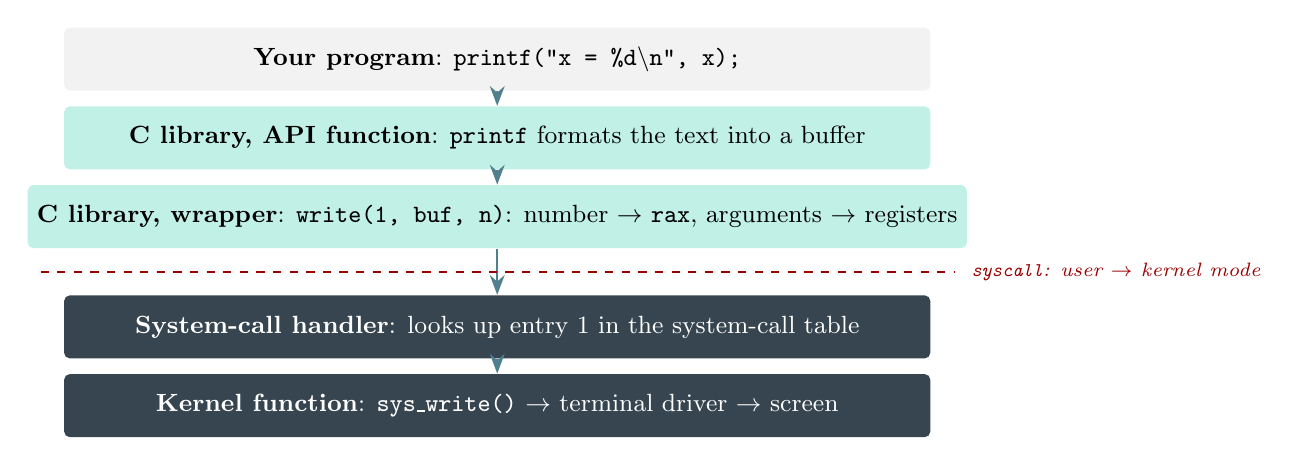
\begin{tikzpicture}[
  l/.style={rectangle,rounded corners=2pt,minimum width=11cm,minimum height=0.8cm,align=center,font=\small},
  arr/.style={-{Stealth[length=2.5mm]},color=slate,thick}]
\node[l,fill=light] (p) at (0,4.0) {\textbf{Your program}: \texttt{printf("x = \%d\textbackslash n", x);}};
\node[l,fill=mint!25] (a) at (0,3.0) {\textbf{C library, API function}: \texttt{printf} formats the text into a buffer};
\node[l,fill=mint!25] (w) at (0,2.0) {\textbf{C library, wrapper}: \texttt{write(1, buf, n)}: number $\to$ \texttt{rax}, arguments $\to$ registers};
\node[l,fill=charcoal,text=white] (h) at (0,0.6) {\textbf{System-call handler}: looks up entry 1 in the system-call table};
\node[l,fill=charcoal,text=white] (k) at (0,-0.4) {\textbf{Kernel function}: \texttt{sys\_write()} $\to$ terminal driver $\to$ screen};
\draw[arr] (p) -- (a); \draw[arr] (a) -- (w); \draw[arr] (w) -- (h); \draw[arr] (h) -- (k);
\draw[dashed,red!60!black,thick] (-5.8,1.3) -- (5.8,1.3);
\node[font=\scriptsize\itshape,text=red!60!black,anchor=west] at (5.9,1.3) {\texttt{syscall}: user $\to$ kernel mode};
\end{tikzpicture}
\caption{From \cmd{printf()} to the screen. Above the dashed line: user mode; below it: kernel mode.}
\end{figure}

Three words are easily confused:

\begin{itemize}
  \item An \term{API} (application programming interface) is a documented set of functions that a programmer can call, together with their parameters and return values. Examples: the \emph{POSIX} API (Linux, macOS, the BSDs), the \emph{Windows API}, and the \emph{Java API}.
  \item A \term{wrapper} is a tiny library function, usually with the same name as the system call (\cmd{write}, \cmd{read}, \cmd{fork}), whose only job is to put the arguments where the kernel expects them and execute the trap instruction.
  \item A \term{system call} is the actual, controlled entry into the kernel.
\end{itemize}

Not every API function makes a system call. \cmd{strlen()} and \cmd{sqrt()} never do: they compute their result in user mode. \cmd{printf()} makes a system call only when its buffer is flushed, so ten calls to \cmd{printf()} may produce a single \cmd{write}. The C library on Linux is usually \emph{glibc}; on Windows, the Windows API functions in \texttt{kernel32.dll} call the native interface in \texttt{ntdll.dll}, which executes the real kernel calls (e.g.\ \cmd{CreateProcess()} eventually calls \cmd{NtCreateUserProcess}).

\subsection{Why program against an API?}

The main reason is \textbf{portability}. A program written for the POSIX API compiles on any POSIX system, whereas system-call \emph{numbers} and details differ between operating systems and even between CPU architectures of the same OS: \cmd{write} is system call number $1$ on 64-bit x86 Linux, $4$ on 32-bit x86 Linux and $64$ on 64-bit ARM Linux, while the API name \cmd{write()} is the same on all three. A second reason is \textbf{convenience}: API functions are easier to use and often add useful work, such as the formatting and buffering of \cmd{printf()}.

\subsection{The system-call number and the system-call table}

Every system call is identified by a small integer, the \term{system-call number}. The kernel keeps a \term{system-call table}: an array, indexed by this number, of pointers to the kernel functions that do the work.

\begin{figure}[H]
\centering
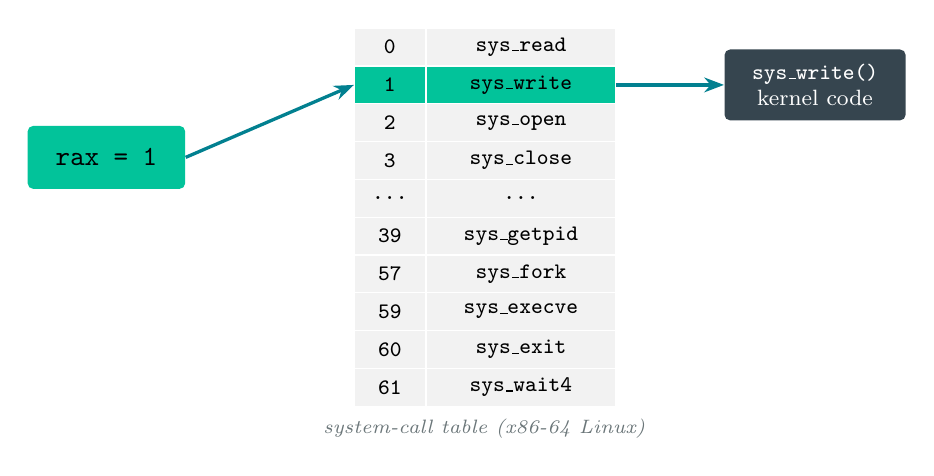
\begin{tikzpicture}[
  c/.style={rectangle,minimum height=0.48cm,font=\footnotesize\ttfamily,draw=white,fill=light},
  arr/.style={-{Stealth[length=2.5mm]},color=mintdeep,very thick}]
\node[rectangle,rounded corners=2pt,fill=mint,minimum width=2cm,minimum height=0.8cm,font=\ttfamily] (r) at (-3.6,0.6) {rax = 1};
\foreach \i/\n/\f/\c in {0/0/sys\_read/light, 1/1/sys\_write/mint, 2/2/sys\_open/light, 3/3/sys\_close/light, 4/\dots/\dots/light, 5/39/sys\_getpid/light, 6/57/sys\_fork/light, 7/59/sys\_execve/light, 8/60/sys\_exit/light, 9/61/sys\_wait4/light} {
  \node[c,minimum width=0.9cm,fill=\c] (n\i) at (0,2.0-\i*0.48) {\n};
  \node[c,minimum width=2.4cm,anchor=west,fill=\c] (f\i) at (n\i.east) {\f};
}
\node[rectangle,rounded corners=2pt,fill=charcoal,text=white,minimum width=2.3cm,minimum height=0.9cm,align=center,font=\footnotesize] (k) at (5.4,1.52) {\texttt{sys\_write()}\\kernel code};
\draw[arr] (r.east) -- (n1.west);
\draw[arr] (f1.east) -- (k.west);
\node[font=\scriptsize\itshape,text=muted] at (1.2,-2.85) {system-call table (x86-64 Linux)};
\end{tikzpicture}
\caption{The number in \texttt{rax} selects an entry of the system-call table. The numbers are the real x86-64 Linux numbers.}
\end{figure}

Why a table, and not simply a jump to the address of \cmd{sys\_write}? Because a user program must \emph{never} be allowed to jump to an arbitrary kernel address: it could skip the permission checks at the start of a kernel function. The trap instruction therefore always enters the kernel at \emph{one} fixed entry point. The kernel checks that the number is valid (an invalid number returns the error \texttt{ENOSYS}) and only then calls the function from the table. Compare this with the interrupt vector of Week~2: both are tables of handler addresses indexed by a number. On our test system (Linux headers for kernel~6.8, x86-64) about $370$ system calls are defined, numbered from $0$ to $461$.

\subsection{The trap, step by step}

Here is what happens when a program calls \cmd{write(1, msg, 26)} on 64-bit x86 Linux:

\begin{enumerate}[leftmargin=1.4em]
  \item \textbf{Load registers} (user mode). The \cmd{write()} wrapper in the C library puts the system-call number $1$ in register \texttt{rax} and the three parameters in \texttt{rdi}, \texttt{rsi} and \texttt{rdx}.
  \item \textbf{Trap.} The wrapper executes the \texttt{syscall} instruction. The CPU switches the mode bit to kernel mode, saves the return address and flags, and jumps to the kernel's single system-call entry point.
  \item \textbf{Save and check} (kernel mode). The kernel saves the user's registers and checks that $1$ is a valid system-call number.
  \item \textbf{Dispatch.} The kernel calls \cmd{sys\_write()} through the table. \cmd{sys\_write()} checks that file descriptor $1$ is open and that the buffer address really belongs to the calling process, then passes the bytes to the terminal driver.
  \item \textbf{Result.} The return value, the number of bytes written ($26$) or a negative error code, is placed in \texttt{rax}.
  \item \textbf{Return.} The \texttt{sysret} instruction restores the user state and switches back to user mode. The wrapper returns $26$ to the program.
\end{enumerate}

The check in step~4 matters: without it, a program could ask the kernel to ``write'' bytes from a kernel address to the screen and so read kernel secrets. A system call is a request, and the kernel trusts nothing in it.

\subsection{Three ways to pass parameters}

A system call usually needs more information than just its number: which file, which buffer, how many bytes. There are three general methods to pass these parameters to the OS.

\begin{figure}[H]
\centering
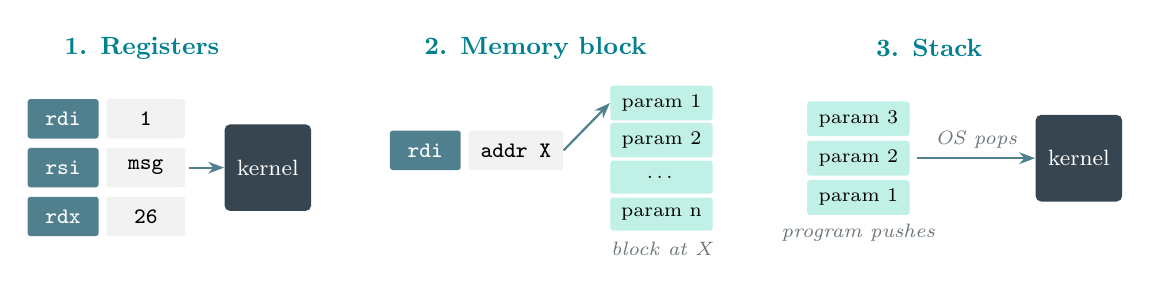
\begin{tikzpicture}[
  r/.style={rectangle,rounded corners=1pt,minimum width=0.9cm,minimum height=0.5cm,font=\footnotesize\ttfamily,fill=slate,text=white},
  v/.style={rectangle,rounded corners=1pt,minimum width=1.0cm,minimum height=0.5cm,font=\footnotesize\ttfamily,fill=light},
  p/.style={rectangle,rounded corners=1pt,minimum width=1.3cm,minimum height=0.42cm,font=\scriptsize,fill=mint!25},
  k/.style={rectangle,rounded corners=2pt,minimum width=1.1cm,minimum height=1.1cm,font=\footnotesize,fill=charcoal,text=white},
  arr/.style={-{Stealth[length=2mm]},color=slate,thick}]
% 1 registers
\node[font=\small\bfseries,text=mintdeep] at (1.0,2.2) {1. Registers};
\foreach \i/\a/\b in {0/rdi/1,1/rsi/msg,2/rdx/26} {\node[r] at (0,1.3-\i*0.62) {\a}; \node[v] at (1.05,1.3-\i*0.62) {\b};}
\node[k] (k1) at (2.6,0.68) {kernel};
\draw[arr] (1.6,0.68) -- (k1.west);
% 2 block
\node[font=\small\bfseries,text=mintdeep] at (6.0,2.2) {2. Memory block};
\node[r] at (4.6,0.9) {rdi}; \node[v,minimum width=1.2cm] (ax) at (5.75,0.9) {addr X};
\foreach \i/\t in {0/param 1,1/param 2,2/\dots,3/param n} \node[p] (b\i) at (7.6,1.5-\i*0.47) {\t};
\node[font=\scriptsize\itshape,text=muted] at (7.6,-0.35) {block at X};
\draw[arr] (ax.east) -- (b0.west);
% 3 stack
\node[font=\small\bfseries,text=mintdeep] at (11.0,2.2) {3. Stack};
\foreach \i/\t in {0/param 3,1/param 2,2/param 1} \node[p] at (10.1,1.3-\i*0.5) {\t};
\node[font=\scriptsize\itshape,text=muted] at (10.1,-0.15) {program pushes};
\node[k] (k3) at (12.9,0.8) {kernel};
\draw[arr] (10.85,0.8) -- node[above,font=\scriptsize\itshape,text=muted]{OS pops} (k3.west);
\end{tikzpicture}
\caption{Three ways of passing parameters to a system call.}
\end{figure}

\begin{enumerate}[leftmargin=1.4em]
  \item \textbf{In registers.} The fastest method: no memory access is needed. Its limit is the number of available registers; x86-64 Linux allows six parameters.
  \item \textbf{In a block (table) in memory.} The program stores the parameters in a block of memory and passes only the block's \emph{address} in a register. Any number of parameters is possible. Linux uses this for system calls with many options; for example, \cmd{clone3()} receives a pointer to a \texttt{struct clone\_args}.
  \item \textbf{On the stack.} The program \emph{pushes} the parameters onto its stack; the OS \emph{pops} (reads) them from there. This was used, for example, by 32-bit FreeBSD on x86.
\end{enumerate}

Methods~2 and~3 have a hidden cost: the kernel must copy the parameters from user memory into kernel memory and check that the addresses really belong to the calling process. Linux combines methods~1 and~2: up to six parameters in registers, and anything larger (a buffer, a structure) passed as an address in a register. Note that even in method~1 the $26$ bytes of the message stay in user memory; only their address travels in a register.

\subsection{Concrete example: the x86-64 Linux convention}

\begin{center}
\renewcommand{\arraystretch}{1.3}
\begin{tabularx}{\linewidth}{>{\ttfamily}l >{\raggedright\arraybackslash}X >{\raggedright\arraybackslash}X}
\toprule
\textrm{\textbf{Register}} & \textbf{Role in a system call} & \textbf{For \texttt{write(1, msg, 26)}} \\
\midrule
rax & system-call number (in), return value (out) & $1$ in, $26$ out (bytes written) \\
rdi & 1st parameter & $1$ (file descriptor: standard output) \\
rsi & 2nd parameter & address of \texttt{msg} \\
rdx & 3rd parameter & $26$ (number of bytes) \\
r10, r8, r9 & 4th, 5th, 6th parameter & not used by \cmd{write} \\
rcx, r11 & overwritten by the \texttt{syscall} instruction & the CPU saves the return address and the flags here \\
\bottomrule
\end{tabularx}
\end{center}

Ordinary C function calls on x86-64 pass the fourth argument in \texttt{rcx}; the system-call convention uses \texttt{r10} instead, because the \texttt{syscall} instruction itself overwrites \texttt{rcx}. A return value between $-4095$ and $-1$ signals an error: the wrapper stores the positive error number in the global variable \texttt{errno} and returns $-1$ to the program. You do not need to memorise the registers; the important idea is that parameters travel in registers.

\subsection{Example 1: the same message, three levels deep}

The programs in this section are in the \texttt{code/} folder next to these notes, with a \texttt{Makefile} (type \cmd{make}). They are written in C for Linux; as in Week~2, you are not expected to write C, only to read the comments and understand what happens. The first program prints three messages: through \cmd{printf()}, through the \cmd{write()} wrapper, and by executing the \texttt{syscall} instruction by hand with a few lines of inline assembly that do exactly what the wrapper does.

\lstinputlisting[caption={}]{../code/raw_write.c}

\begin{lstlisting}[style=term]
$ make raw_write && strace ./raw_write
...
write(1, "1) printf  -> libc -> write\n", 28) = 28
write(1, "2) write() -> libc wrapper\n", 27) = 27
write(1, "3) syscall instruction!!!\n", 26) = 26
write(1, "kernel returned 26 (bytes writte"..., 35) = 35
exit_group(0)                           = ?
\end{lstlisting}

Two observations. First, \cmd{strace} cannot tell the three levels apart: to the kernel, all three are the same system call number~$1$ with three parameters. Second, the kernel returned $26$ in \texttt{rax}, exactly the number of bytes we asked it to write. The inline assembly is for demonstration only and works only on x86-64 Linux; on ARM processors the trap instruction is \texttt{svc} and different registers are used.

\subsection{Six categories of system calls}

System calls can be grouped into six categories. The table gives typical examples; the Windows column lists Windows API functions, each of which calls one or more native system calls.

\begin{center}
\small
\renewcommand{\arraystretch}{1.3}
\begin{tabularx}{\linewidth}{>{\raggedright\arraybackslash}p{2.6cm} >{\raggedright\arraybackslash}p{3.0cm} >{\raggedright\arraybackslash}p{3.3cm} >{\raggedright\arraybackslash}X}
\toprule
\textbf{Category} & \textbf{Typical requests} & \textbf{Linux (POSIX)} & \textbf{Windows API} \\
\midrule
Process control & create, end, load, wait & \cmd{fork()}, \cmd{execve()}, \cmd{exit()}, \cmd{wait4()} & \cmd{CreateProcess()}, \cmd{ExitProcess()}, \cmd{WaitForSingleObject()} \\
File management & create, open, read, write, close & \cmd{open()}, \cmd{read()}, \cmd{write()}, \cmd{close()} & \cmd{CreateFile()}, \cmd{ReadFile()}, \cmd{WriteFile()}, \cmd{CloseHandle()} \\
Device management & request, read, write, configure & \cmd{ioctl()}, \cmd{read()}, \cmd{write()} & \cmd{SetConsoleMode()}, \cmd{ReadConsole()}, \cmd{WriteConsole()} \\
Information maintenance & time, date, IDs, system data & \cmd{getpid()}, \cmd{uname()}, \cmd{clock\_gettime()} & \cmd{GetCurrentProcessId()}, \cmd{GetSystemTime()} \\
Communication & pipes, shared memory, network & \cmd{pipe()}, \cmd{mmap()}, \cmd{socket()} & \cmd{CreatePipe()}, \cmd{MapViewOfFile()} \\
Protection & permissions, ownership & \cmd{chmod()}, \cmd{chown()}, \cmd{umask()} & \cmd{SetFileSecurity()}, \cmd{SetSecurityDescriptorGroup()} \\
\bottomrule
\end{tabularx}
\end{center}

Notice that \cmd{read()} and \cmd{write()} appear under both file and device management. In UNIX a device looks like a special file (for example \texttt{/dev/tty} for the terminal), so the same system calls serve both. This is the extended-machine view of Week~2 at work: one abstraction, many kinds of hardware.

\begin{example}[How many system calls does copying a file take?]
A program that copies one file to another needs, in the classic textbook description:
\begin{enumerate}[leftmargin=1.4em]
  \item Ask for the two file names (I/O system calls, or read them from the command line).
  \item Open the input file; if it does not exist, print an error message and exit (file management, process control).
  \item Create the output file.
  \item Loop: read a block from the input, write it to the output, until \cmd{read()} returns $0$ (end of file).
  \item Close both files, report success, and exit.
\end{enumerate}
With a buffer of $B$ bytes and a file of $S$ bytes, the loop alone makes $\lceil S/B \rceil$ reads that return data, one final read that returns $0$, and $\lceil S/B \rceil$ writes. For $S = 1\ \text{MiB} = 2^{20}$ bytes and $B = 4096 = 2^{12}$ bytes that is $2\cdot 2^{8} + 1 = 513$ system calls.

The real GNU \cmd{cp} (version 9.4) on our test machine behaves differently. \cmd{strace -c cp in.bin out.bin} for a $1$~MiB file counted $102$ system calls in total, the largest groups being \cmd{mmap} ($26$), \cmd{close} ($13$), \cmd{openat} ($11$), \cmd{fstat} ($10$) and \cmd{read} ($9$) --- and just $2$ calls of \cmd{copy\_file\_range}.
Only $2$ of the $102$ calls move data: \cmd{copy\_file\_range} asks the kernel to copy the whole file \emph{inside the kernel}, without passing the bytes through the program's memory. Most of the remaining calls load the program and its shared libraries (\cmd{mmap}, \cmd{openat}, \cmd{read} of library headers). Moving work into the kernel to save system calls is a recurring theme in OS design.
\end{example}

\subsection{System programs}

\term{System programs} (also called system utilities) ship with the OS and provide a convenient environment for program development and execution. They run in user mode and make system calls on your behalf. Most users see the operating system through them, not through system calls. The main categories are: \textbf{file management} (\cmd{ls}, \cmd{cp}, \cmd{rm}, File Explorer); \textbf{status information} (\cmd{date}, \cmd{df}, \cmd{ps}, \cmd{top}, Task Manager, the system logs); \textbf{file modification} (editors such as \cmd{nano} and Notepad, search tools such as \cmd{grep}); \textbf{programming-language support} (compilers, debuggers, interpreters: \cmd{gcc}, \cmd{gdb}, \cmd{python}); \textbf{program loading and execution} (loaders and linkers); \textbf{communications} (\cmd{ssh}, web browsers, e-mail); and \textbf{background services}, programs started at boot that run all the time, called \term{daemons} in UNIX and \emph{services} in Windows (\cmd{sshd}, \cmd{cron}, the print spooler).

Many of these programs will be used hands-on in Weeks~9--14.

% =====================================================================
\section{The Process Concept}
\label{sec:process}

\subsection{Program versus process}

A \term{program} is a \emph{passive} entity: a file on disk containing a list of instructions, such as \texttt{/usr/bin/bash}. A \term{process} is an \emph{active} entity: a program in execution. Besides the program code, a process has
\begin{itemize}
  \item a \emph{current activity}: the value of the \term{program counter} (the address of the next instruction) and of the other CPU registers;
  \item its own \emph{memory}: a stack, a heap and global data (Section~\ref{sec:layout});
  \item resources given to it by the OS: open files, network connections, and so on.
\end{itemize}

A program becomes a process when it is loaded into memory, for example when you double-click an icon or type its name in a shell. One program can be the basis of many processes: if you open two terminal windows, two \texttt{bash} processes run from the same program file, each with its own memory and its own progress. Older books use the word \emph{job} (from batch systems) for the same idea.

\textbf{Analogy:} a recipe is a program; cooking it is a process. Two cooks can follow the same recipe at the same time, each with their own ingredients and their own position in the recipe.

\subsection{A process in memory}
\label{sec:layout}

The memory of a process is divided into regions (also called segments or sections):

\begin{figure}[H]
\centering
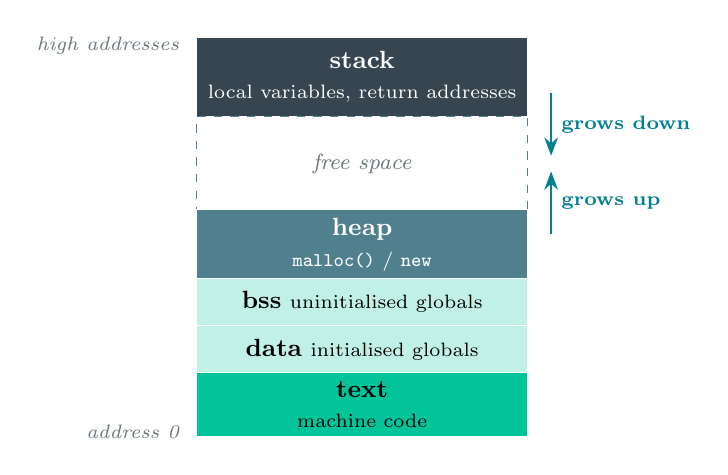
\begin{tikzpicture}[s/.style={rectangle,minimum width=4.2cm,align=center,font=\small,draw=white}]
\node[s,fill=charcoal,text=white,minimum height=1.0cm] (st) at (0,4.6) {\textbf{stack}\\{\scriptsize local variables, return addresses}};
\node[s,draw=slate,dashed,minimum height=1.2cm,font=\footnotesize\itshape,text=muted] (fr) at (0,3.5) {free space};
\node[s,fill=slate,text=white,minimum height=0.85cm] (hp) at (0,2.47) {\textbf{heap}\\{\scriptsize \texttt{malloc()} / \texttt{new}}};
\node[s,fill=mint!25,minimum height=0.6cm] (bs) at (0,1.74) {\textbf{bss} {\scriptsize uninitialised globals}};
\node[s,fill=mint!25,minimum height=0.6cm] (da) at (0,1.14) {\textbf{data} {\scriptsize initialised globals}};
\node[s,fill=mint,minimum height=0.8cm] (tx) at (0,0.44) {\textbf{text}\\{\scriptsize machine code}};
\draw[-{Stealth},thick,mintdeep] (2.4,4.4) -- node[right,font=\scriptsize\bfseries]{grows down} (2.4,3.6);
\draw[-{Stealth},thick,mintdeep] (2.4,2.6) -- node[right,font=\scriptsize\bfseries]{grows up} (2.4,3.4);
\node[font=\scriptsize\itshape,text=muted,anchor=east] at (-2.2,5.0) {high addresses};
\node[font=\scriptsize\itshape,text=muted,anchor=east] at (-2.2,0.1) {address 0};
\end{tikzpicture}
\caption{Layout of a process in memory.}
\end{figure}

\begin{itemize}
  \item \textbf{Text:} the compiled machine code of the program. Read-only, so that a bug cannot overwrite the code; several processes running the same program can share it.
  \item \textbf{Data:} global (and \texttt{static}) variables that have an initial value, e.g.\ \texttt{int initialised = 42;}. The values are stored in the executable file.
  \item \textbf{BSS:} global variables \emph{without} an initial value, e.g.\ \texttt{int uninitialised;}. The OS fills this region with zeros when the program is loaded, so the executable file needs to store only its size. (The name is historical: ``block started by symbol'', from an old assembler.)
  \item \textbf{Heap:} memory requested while the program runs, with \cmd{malloc()} in C or \texttt{new} in C++ and Java. It lives until it is explicitly freed.
  \item \textbf{Stack:} one \emph{frame} per active function call, holding its local variables, parameters and return address. A frame is removed when its function returns.
\end{itemize}

Text, data and bss have a fixed size once the program is loaded; the heap and the stack grow and shrink while it runs, towards each other into the free space between them. A stack that grows too far, for example through infinite recursion, causes a \emph{stack overflow} and the program is terminated.

\subsection{Example 2: printing the address of each region}

\lstinputlisting[caption={}]{../code/mem_layout.c}

\begin{lstlisting}[style=term]
$ ./mem_layout
text  main()        0x555d9ba160c0
data  initialised   0x555d9ba19010
bss   uninitialised 0x555d9ba19018
heap  *dynamic      0x555db649d2a0
stack local         0x7ffe2b4f6ab4
\end{lstlisting}

The order of the addresses matches the figure: text $<$ data $<$ bss $<$ heap, with the stack far above. In the first run the data variable lies $\texttt{0x555d9ba19010} - \texttt{0x555d9ba160c0} = \texttt{0x2f50} = 12\,112$ bytes above \texttt{main}, and the bss variable only $8$ bytes above the data variable: they sit next to each other. The gap between heap and stack is $\texttt{0x7ffe2b4f6ab4} - \texttt{0x555db649d2a0} \approx 4.7\times10^{13}$ bytes, about $43\ \text{TiB}$, far more than the RAM of any PC. This is possible because these are \emph{virtual} addresses; only the parts actually used are backed by physical memory (Week~7).

Run the program again and every address is different: in our second run, for example, \texttt{main} was at \texttt{0x55a4811220c0} and \texttt{local} at \texttt{0x7ffec440c1f4}. Linux places the regions at random positions each time a program starts, a technique called \term{address space layout randomisation} (ASLR). An attacker who finds a bug in a program then cannot know in advance where its code and data are.

\begin{histnote}[ASLR]
ASLR was introduced by the PaX security project for Linux in 2001 and entered the standard Linux kernel in 2005; Windows adopted it with Windows Vista (2007). Today it is standard on desktop and mobile systems.
\end{histnote}

% =====================================================================
\section{Process States}
\label{sec:states}

As a process executes, it changes \term{state}. Each process is in one of five states:

\begin{itemize}
  \item \textbf{New:} the process is being created.
  \item \textbf{Ready:} the process is waiting to be assigned a CPU.
  \item \textbf{Running:} its instructions are being executed.
  \item \textbf{Waiting} (also \emph{blocked}): the process is waiting for some event, such as the completion of an I/O operation or the end of a child process.
  \item \textbf{Terminated:} the process has finished execution.
\end{itemize}

\begin{figure}[H]
\centering
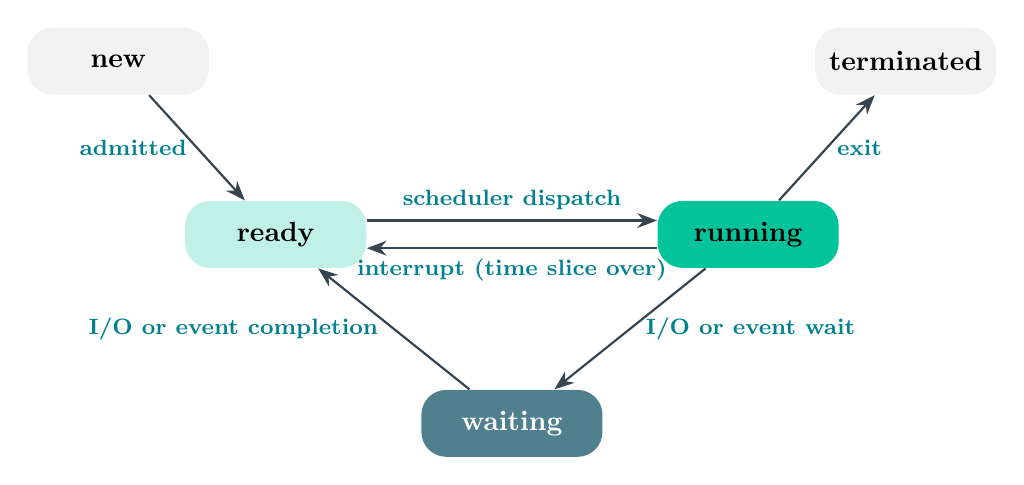
\begin{tikzpicture}[
  st/.style={rectangle,rounded corners=9pt,minimum width=2.3cm,minimum height=0.85cm,font=\headfont\bfseries},
  arr/.style={-{Stealth[length=2.5mm]},thick,charcoal},
  lab/.style={font=\footnotesize\bfseries,text=mintdeep}]
\node[st,fill=light] (new) at (0,3) {new};
\node[st,fill=mint!25] (rdy) at (2,0.8) {ready};
\node[st,fill=mint] (run) at (8,0.8) {running};
\node[st,fill=light] (trm) at (10,3) {terminated};
\node[st,fill=slate,text=white] (wt) at (5,-1.6) {waiting};
\draw[arr] (new) -- node[left,lab]{admitted} (rdy);
\draw[arr] ([yshift=5pt]rdy.east) -- node[above,lab]{scheduler dispatch} ([yshift=5pt]run.west);
\draw[arr] ([yshift=-5pt]run.west) -- node[below,lab]{interrupt (time slice over)} ([yshift=-5pt]rdy.west -| rdy.east);
\draw[arr] (run) -- node[right,lab]{exit} (trm);
\draw[arr] (run) -- node[right,lab,xshift=2pt]{I/O or event wait} (wt);
\draw[arr] (wt) -- node[left,lab,xshift=-2pt]{I/O or event completion} (rdy);
\end{tikzpicture}
\caption{The five-state process model.}
\end{figure}

Only one process can be \emph{running} on a CPU core at any instant; many processes may be \emph{ready} or \emph{waiting}. The OS keeps the ready processes in a \term{ready queue} and the waiting processes in \term{wait queues} (one per device or event); each queue is a linked list of process control blocks (Section~\ref{sec:pcb}).

\subsection{What triggers each transition}

\begin{center}
\renewcommand{\arraystretch}{1.3}
\begin{tabularx}{\linewidth}{>{\raggedright\arraybackslash}p{3.2cm} >{\raggedright\arraybackslash}X >{\raggedright\arraybackslash}p{4.6cm}}
\toprule
\textbf{Transition} & \textbf{Triggered by} & \textbf{Everyday example} \\
\midrule
new $\to$ ready & the OS has created the PCB and loaded the program & you type \cmd{./mem\_layout} and press Enter \\
ready $\to$ running & the scheduler \emph{dispatches} the process & a CPU core becomes free and the scheduler picks it \\
running $\to$ ready & an interrupt, usually the timer (time slice used up) & a long calculation is paused so that others can run \\
running $\to$ waiting & a system call that must wait (I/O, child, sleep) & \cmd{read()} from the disk; \cmd{wait()} for a child \\
waiting $\to$ ready & the awaited event happens, often signalled by an interrupt & the disk interrupt says the data has arrived \\
running $\to$ terminated & \cmd{exit()} or a fatal error & \cmd{main()} returns; the program divides by zero \\
\bottomrule
\end{tabularx}
\end{center}

Two remarks. First, a process can never go from \emph{waiting} directly to \emph{running}: when its event happens it joins the ready queue and must wait until the scheduler dispatches it. Which ready process runs next is the subject of \emph{CPU scheduling} (Weeks~4--5). Second, notice who causes the transitions: a process leaves the running state either by making a system call (Section~\ref{sec:syscalls}) or because an interrupt (Week~2) takes the CPU away. The OS is interrupt-driven.

On Linux, the \cmd{ps} command shows the state in its \texttt{STAT} column: \texttt{R} for running \emph{or} ready (Linux does not distinguish them there), \texttt{S} for sleeping (waiting, interruptible), \texttt{D} for waiting uninterruptibly (usually for disk I/O), \texttt{T} for stopped and \texttt{Z} for zombie (Section~\ref{sec:zombie}).

\begin{example}[Two processes, one CPU]
Process A computes for $3$~ms, reads from the disk ($4$~ms), then computes for $2$~ms more. Process B needs $7$~ms of CPU time. The OS gives each process a time slice of at most $5$~ms. Both are ready at $t = 0$, and A is dispatched first.

\begin{center}
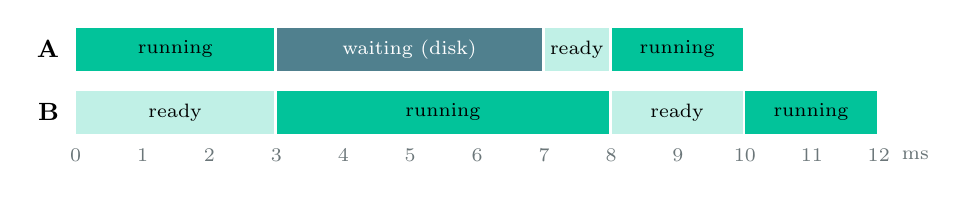
\begin{tikzpicture}[x=0.85cm,y=1cm,g/.style={rectangle,minimum height=0.55cm,font=\scriptsize,anchor=west,inner sep=0pt}]
\foreach \a/\b/\t/\c/\tc in {0/3/running/mint/black, 3/7/{waiting (disk)}/slate/white, 7/8/ready/mint!25/black, 8/10/running/mint/black}
  \node[g,fill=\c,text=\tc,minimum width={(\b-\a)*0.85cm-1pt}] at (\a,1) {\t};
\foreach \a/\b/\t/\c/\tc in {0/3/ready/mint!25/black, 3/8/running/mint/black, 8/10/ready/mint!25/black, 10/12/running/mint/black}
  \node[g,fill=\c,text=\tc,minimum width={(\b-\a)*0.85cm-1pt}] at (\a,0.2) {\t};
\node[anchor=east,font=\small\bfseries] at (-0.1,1) {A};
\node[anchor=east,font=\small\bfseries] at (-0.1,0.2) {B};
\foreach \t in {0,...,12} \node[font=\scriptsize,text=muted] at (\t,-0.35) {\t};
\node[font=\scriptsize,text=muted,anchor=west] at (12.2,-0.35) {ms};
\end{tikzpicture}
\end{center}

\begin{itemize}
  \item $t = 3$: A calls \cmd{read()} and becomes \emph{waiting}; B is dispatched.
  \item $t = 7$: the disk interrupt moves A to \emph{ready}; B keeps the CPU.
  \item $t = 8$: the timer interrupt ends B's $5$~ms slice; B becomes ready and A is dispatched.
  \item $t = 10$: A exits; B runs its remaining $2$~ms and exits at $t = 12$.
\end{itemize}
The CPU work needed is $3 + 2 = 5$~ms for A and $7$~ms for B, $12$~ms in total. Run one after the other, A would take $3 + 4 + 2 = 9$~ms (with the CPU idle for $4$~ms) and B another $7$~ms: $16$~ms in total, with the CPU busy $12/16 = 75\%$ of the time. Interleaved as above, both finish after $12$~ms and the CPU is busy $12/12 = 100\%$ of the time. This is the multiprogramming idea of Week~1, now described with process states.
\end{example}

% =====================================================================
\section{The Process Control Block}
\label{sec:pcb}

Each process is represented in the OS by a \term{process control block} (PCB), also called a \emph{task control block}. It is a data structure in kernel memory that holds everything the OS needs to know about the process.

\begin{figure}[H]
\centering
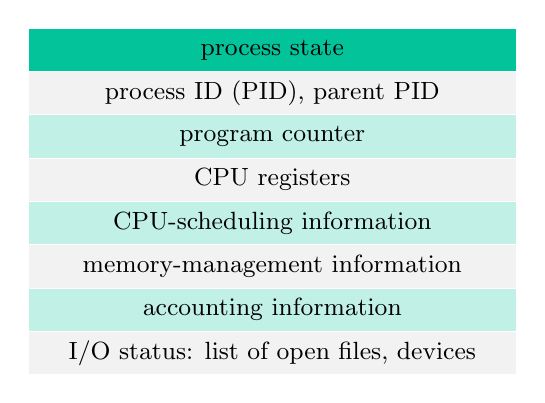
\begin{tikzpicture}[f/.style={rectangle,minimum width=6.2cm,minimum height=0.55cm,font=\small,draw=white}]
\foreach \i/\t/\c in {0/process state/mint, 1/{process ID (PID), parent PID}/light, 2/program counter/mint!25, 3/CPU registers/light, 4/CPU-scheduling information/mint!25, 5/memory-management information/light, 6/accounting information/mint!25, 7/{I/O status: list of open files, devices}/light}
  \node[f,fill=\c] at (0,-\i*0.55) {\t};
\end{tikzpicture}
\caption{Typical contents of a process control block.}
\end{figure}

\begin{itemize}
  \item \textbf{Process state:} new, ready, running, waiting or terminated.
  \item \textbf{Identification:} the process ID (PID), the parent's PID, the owner (user ID).
  \item \textbf{Program counter:} the address of the next instruction to execute.
  \item \textbf{CPU registers:} their values must be saved when the process stops running, so that it can continue correctly later.
  \item \textbf{CPU-scheduling information:} priority, pointers into the scheduling queues.
  \item \textbf{Memory-management information:} where the regions of the process are, e.g.\ base and limit registers or page tables (Weeks~6--7).
  \item \textbf{Accounting information:} CPU time used, time limits, number of context switches.
  \item \textbf{I/O status information:} the list of open files and allocated devices.
\end{itemize}

When a process is not running, its PCB \emph{is} the process as far as the CPU is concerned: it contains everything needed to resume it. In Linux the PCB is a C structure called \texttt{struct task\_struct}, defined in the kernel source file \texttt{include/linux/sched.h}; it has hundreds of fields.

\subsection{Peeking at a PCB: \texttt{/proc/<pid>/status}}

Linux makes parts of every PCB visible as text files in the \texttt{/proc} directory. \texttt{/proc} is not a real directory on disk: the kernel generates the text on the fly when you read it. For a \cmd{sleep} process on our test machine (the \cmd{grep} pattern is broken over two lines here; type it on one line):

\begin{lstlisting}[style=term]
$ sleep 30 &
$ grep -E "^(Name|State|Pid|PPid|Uid|VmSize|VmRSS|Threads|voluntary)" \
       /proc/$!/status
Name:   sleep
State:  S (sleeping)
Pid:    27271
PPid:   27265
Uid:    0       0       0       0
VmSize:     2724 kB
VmRSS:      1696 kB
Threads:        1
voluntary_ctxt_switches:        2
nonvoluntary_ctxt_switches:     0
\end{lstlisting}

\verb|$!| is the PID of the most recent background command. The fields map directly onto the PCB: \texttt{State} is the process state (\cmd{sleep} waits for a timer, so it is \texttt{S}); \texttt{Pid} and \texttt{PPid} identify the process and its parent; \texttt{Uid} is the owner (here user~$0$, the administrator \texttt{root}); \texttt{VmSize} (virtual memory size) and \texttt{VmRSS} (the part actually in RAM) are memory-management information; the two context-switch counters are accounting information. \emph{Voluntary} switches happen when the process gives up the CPU by waiting; \emph{non-voluntary} switches happen when the OS takes the CPU away. The \texttt{Threads} line is next week's topic.

% =====================================================================
\section{Context Switch}
\label{sec:ctx}

When an interrupt or a system call causes the OS to take the CPU from one process and give it to another, the OS performs a \term{context switch}. The \emph{context} of a process is represented in its PCB: the program counter, the CPU registers, the stack pointer, the process state and the memory-management information (which page table is active). A context switch consists of two steps:

\begin{enumerate}[leftmargin=1.4em]
  \item \textbf{State save:} store the context of the current process in its PCB.
  \item \textbf{State restore:} load the context of the next process from its PCB.
\end{enumerate}

\begin{figure}[H]
\centering
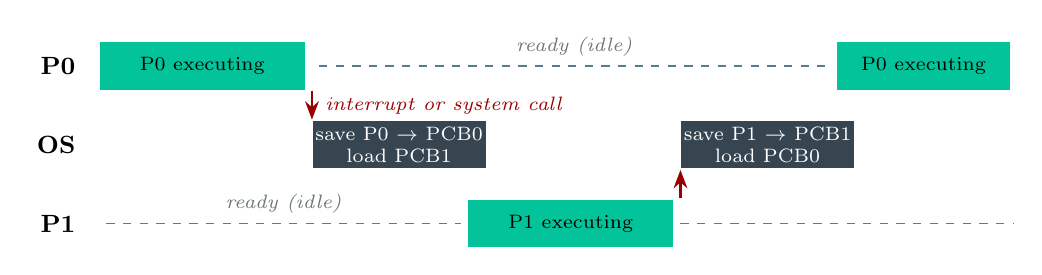
\begin{tikzpicture}[x=0.9cm,y=1cm,g/.style={rectangle,minimum height=0.6cm,font=\scriptsize,anchor=west,inner sep=1pt,align=center}]
\node[anchor=east,font=\small\bfseries] at (-0.2,2) {P0};
\node[anchor=east,font=\small\bfseries] at (-0.2,1) {OS};
\node[anchor=east,font=\small\bfseries] at (-0.2,0) {P1};
\node[g,fill=mint,minimum width=2.6cm] at (0,2) {P0 executing};
\node[g,fill=charcoal,text=white,minimum width=2.1cm] at (3,1) {save P0 $\to$ PCB0\\load PCB1};
\node[g,fill=mint,minimum width=2.6cm] at (5.2,0) {P1 executing};
\node[g,fill=charcoal,text=white,minimum width=2.1cm] at (8.2,1) {save P1 $\to$ PCB1\\load PCB0};
\node[g,fill=mint,minimum width=2.2cm] at (10.4,2) {P0 executing};
\draw[dashed,slate] (3.1,2) -- node[above,font=\scriptsize\itshape,text=muted]{ready (idle)} (10.3,2);
\draw[dashed,slate] (0.1,0) -- node[above,font=\scriptsize\itshape,text=muted]{ready (idle)} (5.1,0);
\draw[dashed,slate] (8.2,0) -- (12.9,0);
\draw[-{Stealth},thick,red!60!black] (3,1.68) -- (3,1.32);
\draw[-{Stealth},thick,red!60!black] (8.2,0.32) -- (8.2,0.68);
\node[font=\scriptsize\itshape,text=red!60!black,anchor=west] at (3.05,1.5) {interrupt or system call};
\end{tikzpicture}
\caption{A context switch from P0 to P1 and back (after Silberschatz et al., Fig.~3.6, drawn with time running left to right).}
\end{figure}

During the switch (the dark boxes) \emph{no process does useful work}: the context switch is pure \term{overhead}. Its direct cost on modern hardware is a few microseconds; it depends on the CPU speed, the number of registers to copy and the memory-management work. There is also a hidden indirect cost: after a switch, the CPU caches and the TLB (Week~6) are full of the previous process's data, so the new process runs more slowly for a while.

\begin{example}[How much does context switching cost?]
Suppose every process runs for a time slice $q$ before the OS switches, and each switch costs $s$. Of every period $q + s$, only $q$ is useful, so the fraction of CPU time lost is
\[
\text{overhead} = \frac{s}{q + s}.
\]
Take $s = 5\ \mu\text{s}$ (an illustrative value):
\begin{center}
\renewcommand{\arraystretch}{1.25}
\begin{tabular}{@{}rrr@{}}
\toprule
\textbf{Time slice $q$} & \textbf{Overhead $s/(q+s)$} & \textbf{Useful work} \\
\midrule
$100$ ms & $0.005\%$ & $99.995\%$ \\
$10$ ms & $0.05\%$ & $99.95\%$ \\
$1$ ms & $0.50\%$ & $99.50\%$ \\
$0.1$ ms & $4.76\%$ & $95.24\%$ \\
$0.01$ ms & $33.3\%$ & $66.7\%$ \\
$0.005$ ms ($q = s$) & $50\%$ & $50\%$ \\
\bottomrule
\end{tabular}
\end{center}
For example, with $q = 1\ \text{ms} = 1000\ \mu\text{s}$: $5/(1000+5) = 0.004975 \approx 0.50\%$. Equivalently, $1000$ switches per second cost $1000 \times 5\ \mu\text{s} = 5\ \text{ms}$ of every second, i.e.\ $0.5\%$.

The lesson: short time slices make the system feel responsive but waste CPU time on switching; long time slices waste little but make interactive programs feel sluggish. Choosing $q$ is a central question of Round-Robin scheduling in Week~5.
\end{example}

% =====================================================================
\section{Process Creation and Termination}
\label{sec:creation}

\subsection{fork(), exec() and wait()}

A process can create new processes. The creator is the \term{parent process}; the new processes are its \term{child processes}. In UNIX and Linux, three system calls do the work:

\begin{itemize}
  \item \cmd{fork()} creates a new process that is an almost exact \emph{copy} of the caller: same program, same memory contents, same open files. The only difference is the return value: \cmd{fork()} returns $0$ in the child and the child's PID in the parent (or $-1$ if no process could be created). It is called once and returns twice.
  \item \cmd{exec()} (in Linux the system call \cmd{execve()}, with library variants such as \cmd{execlp()}) \emph{replaces} the program running in the calling process by a new program. The PID stays the same; the old code, data, heap and stack are discarded. On success \cmd{exec()} never returns.
  \item \cmd{wait()} (or \cmd{waitpid()}) puts the parent into the \emph{waiting} state until a child terminates, and then collects the child's exit status.
\end{itemize}

\begin{figure}[H]
\centering
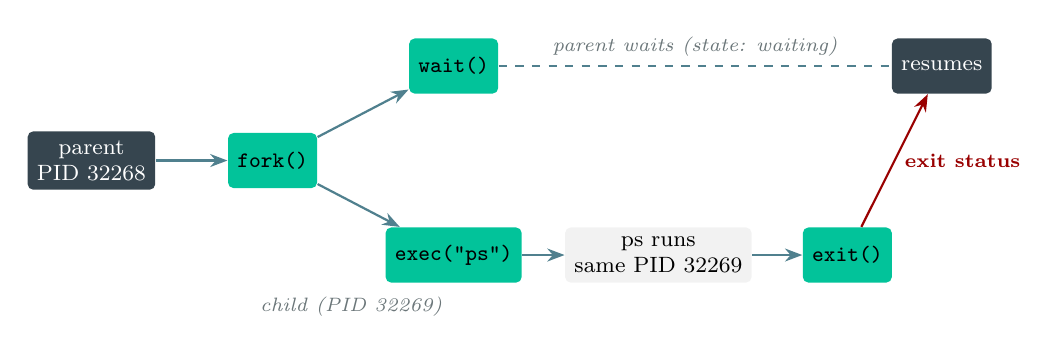
\begin{tikzpicture}[
  b/.style={rectangle,rounded corners=2pt,minimum height=0.7cm,font=\footnotesize,align=center},
  arr/.style={-{Stealth[length=2.2mm]},thick,slate}]
\node[b,fill=charcoal,text=white] (p) at (0,0) {parent\\PID 32268};
\node[b,fill=mint,font=\footnotesize\ttfamily] (f) at (2.3,0) {fork()};
\node[b,fill=mint,font=\footnotesize\ttfamily] (w) at (4.6,1.2) {wait()};
\node[b,fill=charcoal,text=white] (r) at (10.8,1.2) {resumes};
\node[b,fill=mint,font=\footnotesize\ttfamily] (e) at (4.6,-1.2) {exec("ps")};
\node[b,fill=light] (ps) at (7.2,-1.2) {ps runs\\same PID 32269};
\node[b,fill=mint,font=\footnotesize\ttfamily] (x) at (9.6,-1.2) {exit()};
\draw[arr] (p) -- (f); \draw[arr] (f) -- (w); \draw[arr] (f) -- (e);
\draw[arr] (e) -- (ps); \draw[arr] (ps) -- (x);
\draw[dashed,slate] (w) -- node[above,font=\scriptsize\itshape,text=muted]{parent waits (state: waiting)} (r);
\draw[arr,red!60!black] (x) -- node[right,font=\scriptsize\bfseries]{exit status} (r);
\node[font=\scriptsize\itshape,text=muted] at (3.3,-1.85) {child (PID 32269)};
\end{tikzpicture}
\caption{Process creation with \cmd{fork()}, \cmd{exec()} and \cmd{wait()}. PIDs from the real run below.}
\end{figure}

This is exactly what a shell does for every command you type: it forks a copy of itself, the copy (the child) execs the command, and the shell waits for it to finish before printing the next prompt. Why two separate steps? Between \cmd{fork()} and \cmd{exec()}, the child can prepare its environment, for example redirect its output into a file. We will use this in Week~12 (pipes and redirection). Windows combines both steps in one call, \cmd{CreateProcess()}, which takes the name of the program to run as a parameter.

\subsection{Example 3: fork, exec and wait in C}

The listing shows the heart of \texttt{code/fork\_exec\_wait.c}; the full file adds the \texttt{\#include} lines and an error check for a failed \cmd{fork()} (which returns $-1$).

\lstinputlisting[caption={}]{../code/fork_exec_wait_excerpt.c}

\begin{lstlisting}[style=term]
$ ./fork_exec_wait
parent: my PID is 32268
child : PID 32269, my parent is 32268
  PID  PPID STAT COMMAND
32268 32251 S    fork_exec_wait
32269 32268 R    ps
parent: child 32269 finished, exit status 0
\end{lstlisting}

The same \texttt{if} test gives two different answers: the child sees \texttt{pid == 0}, the parent sees the child's PID. The \cmd{ps} output, printed by the child after \cmd{exec()}, lists PID $32269$ as \texttt{ps}: the process kept its PID but now runs a different program. Its state is \texttt{R} (it is running: it is the process doing the listing), while the parent is \texttt{S}, waiting in \cmd{waitpid()}.

Under \cmd{strace -f} the three calls appear as \cmd{clone(\dots) = 6411}, \cmd{execve("/usr/bin/ps", \dots) = 0} and \cmd{wait4(6411, \dots) = 6411} (from another run): the C library implements \cmd{fork()} with the more general Linux system call \cmd{clone()}.

\begin{tryit}[Why the \texttt{fflush(stdout)} before \texttt{fork()}?]
\cmd{printf()} collects text in a buffer inside the process's memory. \cmd{fork()} copies that memory, including any text not yet written. Remove the first \cmd{fflush(stdout)}, run \cmd{./fork\_exec\_wait > out.txt} (output to a file is fully buffered), and look at \texttt{out.txt}: the line ``parent: my PID is \dots'' appears twice, once printed by each process.
\end{tryit}


\subsection{The process tree and process identifiers}

Every process has a unique integer \term{process identifier} (PID) and knows the PID of its parent (PPID). Because every process except the first is created by another, the processes form a \term{process tree}. On Linux the root of the user-space tree is PID~$1$, called \cmd{systemd} (or \cmd{init} on older and smaller systems), which the kernel starts at the end of booting; kernel threads hang below a separate root, \cmd{kthreadd} (PID~$2$).

\begin{figure}[H]
\centering
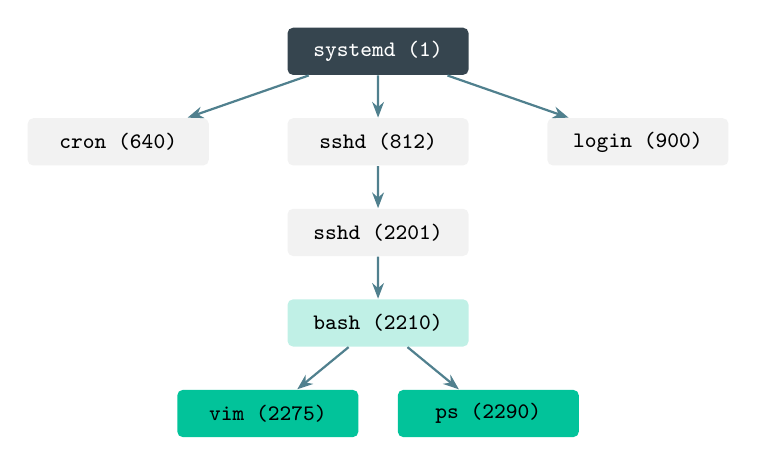
\begin{tikzpicture}[
  n/.style={rectangle,rounded corners=2pt,minimum width=2.3cm,minimum height=0.6cm,font=\footnotesize\ttfamily,fill=light},
  arr/.style={-{Stealth[length=2mm]},slate,thick}, level distance=1.15cm,
  level 1/.style={sibling distance=3.3cm}, level 2/.style={sibling distance=2.8cm}, edge from parent/.style={draw,arr}]
\node[n,fill=charcoal,text=white] {systemd (1)}
  child {node[n] {cron (640)}}
  child {node[n] {sshd (812)}
    child {node[n] {sshd (2201)}
      child {node[n,fill=mint!25] {bash (2210)}
        child {node[n,fill=mint] {vim (2275)}}
        child {node[n,fill=mint] {ps (2290)}}}}}
  child {node[n] {login (900)}};
\end{tikzpicture}
\caption{Part of a typical Linux process tree (PIDs illustrative). A user logged in over SSH runs \cmd{vim} and \cmd{ps} from a \cmd{bash} shell.}
\end{figure}

The command \cmd{pstree -p} draws the real tree. On our test machine:
\begin{lstlisting}[style=term]
$ bash -c 'sleep 5 & sleep 5 & pstree -p $$'
bash(6297)-+-pstree(6300)
           |-sleep(6298)
           `-sleep(6299)
\end{lstlisting}
\verb|$$| is the PID of the shell itself. The new \cmd{bash} created three children, all forked from it. PIDs are assigned in increasing order and reused after a process has ended; the largest PID is configured in \nolinkurl{/proc/sys/kernel/pid_max} ($32768$ on our test machine).

\subsection{Process termination, zombies and orphans}
\label{sec:zombie}

A process terminates when it calls \cmd{exit()} (returning from \cmd{main()} does this implicitly) or when the OS kills it after a fatal error. The OS then frees its memory and closes its files. But the PCB entry with the PID and the \emph{exit status} must survive until the parent collects it with \cmd{wait()}.

\begin{itemize}
  \item A \term{zombie} is a process that has terminated but whose parent has not yet called \cmd{wait()}. It uses no memory or CPU, but it occupies an entry in the process table and keeps its PID. A parent that creates many children and never waits for them can fill the process table, so that no new processes can be created.
  \item An \term{orphan} is a process whose parent terminated first. Linux \emph{re-parents} orphans to PID~$1$ (or to a designated ``subreaper'' process), which calls \cmd{wait()} regularly, so orphans never remain zombies for long. Some systems instead terminate all children when a parent ends (\emph{cascading termination}).
\end{itemize}

A zombie is easy to produce with a shell trick: \cmd{sh -c 'sleep 1 \& exec sleep 4'} starts \cmd{sleep 1} in the background and then \emph{replaces} the shell by \cmd{sleep 4}, a program that never calls \cmd{wait()}. Two seconds later, on our test machine:

\begin{lstlisting}[style=term]
$ ps -o pid,ppid,stat,cmd -p 6385 --ppid 6385
  PID  PPID STAT CMD
 6385  6384 S    sleep 4
 6387  6385 Z    [sleep] <defunct>
\end{lstlisting}

The finished \cmd{sleep 1} is shown in state \texttt{Z} and marked \texttt{<defunct>}. When \cmd{sleep 4} ends two seconds later, the zombie becomes an orphan, is adopted by its new parent and is reaped.

\subsection{Example 4: how many processes after $n$ calls to fork()?}

The program \texttt{code/fork\_count.c} reads $n$ from the command line and then executes
\begin{lstlisting}
for (int i = 0; i < n; i++)
    fork();                   /* parent AND child continue */
printf("PID %6d  parent %6d\n", getpid(), getppid());
while (wait(NULL) > 0)        /* reap all children: no zombies */
    ;
\end{lstlisting}

Every \emph{existing} process executes each subsequent \cmd{fork()}. Before the first fork there is $1$ process; after it, $2$; after the second, $4$; after the $n$-th, $2^{n}$. Of these, $2^{n} - 1$ were created by \cmd{fork()} (all except the original), and the \cmd{printf} runs $2^{n}$ times. A real run with $n = 3$:

\begin{lstlisting}[style=term]
$ ./fork_count 3
PID   1939  parent   1937
PID   1938  parent   1937
PID   1940  parent   1937
PID   1941  parent   1938
PID   1942  parent   1939
PID   1943  parent   1938
PID   1937  parent   1903
PID   1944  parent   1941
\end{lstlisting}

Eight lines, from eight different processes. The parent column reveals the tree: the original process $1937$ created $1938$, $1939$ and $1940$ in forks $1$, $2$ and $3$; $1938$ (born in fork~$1$) itself executed forks~$2$ and~$3$, creating $1941$ and $1943$; and so on. The order of the lines changes from run to run, because the scheduler decides which process runs first.

\begin{figure}[H]
\centering
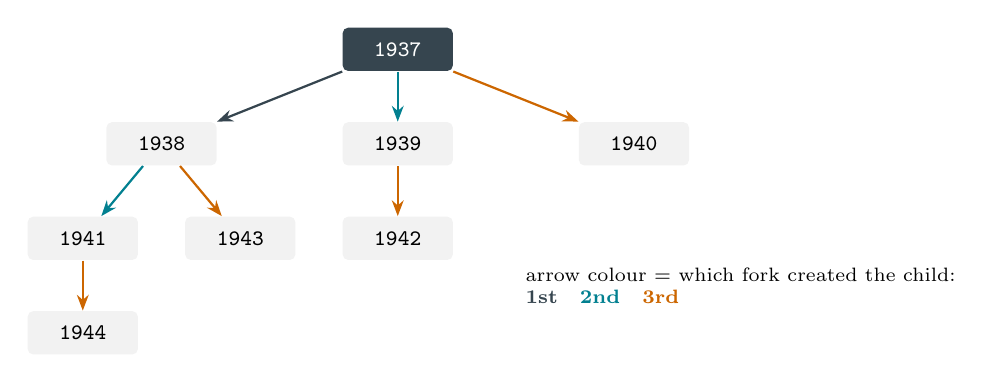
\begin{tikzpicture}[
  n/.style={rectangle,rounded corners=2pt,minimum width=1.4cm,minimum height=0.55cm,font=\footnotesize\ttfamily,fill=light},
  e1/.style={-{Stealth[length=2mm]},thick,charcoal}, e2/.style={-{Stealth[length=2mm]},thick,mintdeep}, e3/.style={-{Stealth[length=2mm]},thick,orange!80!black}]
\node[n,fill=charcoal,text=white] (r) at (0,0) {1937};
\node[n] (a) at (-3,-1.2) {1938}; \node[n] (b) at (0,-1.2) {1939}; \node[n] (c) at (3,-1.2) {1940};
\node[n] (d) at (-4,-2.4) {1941}; \node[n] (e) at (-2,-2.4) {1943}; \node[n] (f) at (0,-2.4) {1942};
\node[n] (g) at (-4,-3.6) {1944};
\draw[e1] (r) -- (a); \draw[e2] (r) -- (b); \draw[e3] (r) -- (c);
\draw[e2] (a) -- (d); \draw[e3] (a) -- (e); \draw[e3] (b) -- (f); \draw[e3] (d) -- (g);
\node[font=\scriptsize,anchor=west,align=left] at (1.5,-3.0) {arrow colour = which fork created the child:\\{\color{charcoal}\textbf{1st}}\quad{\color{mintdeep}\textbf{2nd}}\quad{\color{orange!80!black}\textbf{3rd}}};
\end{tikzpicture}
\caption{The process tree of \cmd{./fork\_count 3}, with the real PIDs.}
\end{figure}

The formula can be verified by counting output lines:
\begin{lstlisting}[style=term]
$ for n in 0 1 2 3 4 5 6 7 8 9 10; do ./fork_count $n | wc -l; done | tr '\n' ' '
1 2 4 8 16 32 64 128 256 512 1024
\end{lstlisting}

The program refuses $n > 10$ for a good reason: a loop that forks without limit (a ``fork bomb'') fills the process table within seconds. Linux limits the number of processes per user (\cmd{ulimit -u}), an example of the resource-allocation service of Section~\ref{sec:services}.

% =====================================================================
\section{Summary}

\begin{keyidea}[Week 3 in seven sentences]
\begin{enumerate}[leftmargin=1.4em]
  \item The OS offers services for the user (user interface, program execution, I/O, file systems, communication, error detection) and for itself (resource allocation, accounting, protection and security).
  \item Programs reach these services through system calls, normally via an API and a thin library wrapper; the shell and the other system programs are ordinary user-mode programs.
  \item Each system call has a number; the trap instruction enters the kernel at one fixed point, and the kernel uses the number as an index into the system-call table.
  \item Parameters are passed in registers, in a memory block whose address is in a register, or on the stack; x86-64 Linux uses \texttt{rax} for the number and up to six registers for parameters.
  \item A process is a program in execution, with text, data, bss, heap and stack regions, and is described by its process control block.
  \item A process moves between the states new, ready, running, waiting and terminated; system calls and interrupts cause the transitions.
  \item A context switch saves one PCB and loads another and is pure overhead, $s/(q+s)$; processes are created with \cmd{fork()}, \cmd{exec()} and \cmd{wait()}, and $n$ forks in a loop give $2^{n}$ processes.
\end{enumerate}
\end{keyidea}

% =====================================================================
\Needspace{6\baselineskip}
\section{Glossary}

\begin{description}[leftmargin=1em,itemsep=0.1em]
  \item[API] Application programming interface: a documented set of functions that programs can call, e.g.\ POSIX or the Windows API.
  \item[ASLR] Address space layout randomisation: placing the regions of a process at random addresses at every start.
  \item[BSS] The region holding global variables without an initial value; filled with zeros at load time.
  \item[Context switch] Saving the state of the running process in its PCB and loading the state of another process from its PCB.
  \item[Daemon] A background system program, started at boot, that runs without a user interface (a ``service'' on Windows).
  \item[Orphan] A process whose parent has terminated; on Linux it is adopted by PID~1 or a subreaper.
  \item[PCB] Process control block: the kernel data structure that represents one process.
  \item[PID] Process identifier: the unique number of a process.
  \item[Process] A program in execution.
  \item[Ready queue] The list of processes that are ready to run and waiting for a CPU.
  \item[Shell] A command interpreter; a system program that reads commands and runs them.
  \item[System call] A controlled request from a program to the kernel, entered with a trap instruction.
  \item[System-call table] The kernel's array of handler addresses, indexed by system-call number.
  \item[System program] A user-mode program shipped with the OS (file manager, compiler, \cmd{ls}, \cmd{ps}).
  \item[Wrapper] A small library function that loads the registers and executes the trap for one system call.
  \item[Zombie] A terminated process whose exit status has not yet been collected by its parent.
\end{description}

% =====================================================================
\section{Try It Yourself}

\begin{tryit}[Look at processes on your own machine]
\textbf{Linux} (lab PCs, WSL, or a virtual machine):
\begin{lstlisting}[style=term]
$ ps -ef | head            # all processes, with their PPID
$ ps -o pid,ppid,stat,cmd  # your processes and their states
$ pstree -p | less         # the process tree
$ cat /proc/$$/status      # the PCB of your own shell
$ strace -c ls             # system calls of ls, counted by type
$ make && ./fork_count 4   # in the Week 3 code folder
\end{lstlisting}
\textbf{Windows:} run \cmd{tasklist} in a Command Prompt; in Task Manager open the \emph{Details} tab and show the PID column.
\begin{enumerate}[leftmargin=1.4em]
  \item What is the PID of your shell, and which process is its parent?
  \item How many processes are in state \texttt{R} right now? Why are there so few?
  \item How many voluntary context switches has your shell made so far? Run a few commands and look again.
\end{enumerate}
\end{tryit}

% =====================================================================
\section{Review Questions}

\subsection*{Conceptual}
\begin{enumerate}[leftmargin=1.6em]
  \item Explain the difference between an API function, a wrapper and a system call, using \cmd{printf()} and \cmd{write()} as examples. Does \cmd{strlen()} make a system call?
  \item Describe the three methods of passing parameters to the OS. Which does Linux on x86-64 use, and why does it need two of them?
  \item Classify each system call into one of the six categories: \cmd{fork()}, \cmd{chmod()}, \cmd{ioctl()}, \cmd{getpid()}, \cmd{socket()}, \cmd{close()}.
  \item In which memory region does each of these live: a global \texttt{int count;}, a global \texttt{int max = 100;}, a local variable of \cmd{main()}, the memory returned by \cmd{malloc()}, the code of \cmd{main()}?
  \item Draw the five-state diagram. For each transition, name an event that causes it. Why is there no arrow from waiting to running?
  \item What is the difference between \cmd{fork()} and \cmd{exec()}? What does \cmd{fork()} return, and to whom?
  \item What is a zombie process? What is an orphan? How does Linux make sure orphans do not remain zombies?
\end{enumerate}

\subsection*{Numerical}
\begin{enumerate}[leftmargin=1.6em,resume]
  \item A context switch takes $10\ \mu$s. What percentage of CPU time is overhead if the time slice is (a) $1$~ms, (b) $50\ \mu$s?
  \item A system performs $2000$ context switches per second, each costing $4\ \mu$s. What fraction of the CPU is lost? How many CPU-seconds is that per hour?
  \item How many processes exist after this code runs, and how many times is \texttt{"hi"} printed?\\ \texttt{fork(); fork(); fork(); fork(); printf("hi\textbackslash n");}
  \item Process A computes for $2$~ms, waits for the disk for $6$~ms, then computes for $2$~ms. Process B computes for $4$~ms. Both are ready at $t = 0$, A runs first, there is one CPU and no time slice limit. Compute the total time and the CPU utilisation (a) if B starts only after A has finished, (b) if B runs while A waits.
  \item On x86-64 Linux, a program calls \cmd{write(2, "Error\textbackslash n", 6)}. What values are in \texttt{rax}, \texttt{rdi} and \texttt{rdx} just before the \texttt{syscall} instruction, and what is in \texttt{rax} afterwards if all bytes are written?
\end{enumerate}

\subsection*{Answers to the numerical questions}
\begin{enumerate}[leftmargin=1.6em,start=8]
  \item (a) $10/(1000 + 10) \approx 0.0099 = 0.99\%$, about $1\%$. (b) $10/(50 + 10) \approx 0.167 = 16.7\%$: one sixth of the CPU is wasted.
  \item $2000\ \text{s}^{-1} \times 4\times10^{-6}\ \text{s} = 8\times10^{-3} = 0.8\%$. Per hour: $0.008 \times 3600\ \text{s} = 28.8$ CPU-seconds.
  \item Four forks: $2^{4} = 16$ processes ($15$ created), and \texttt{"hi"} is printed $16$ times.
  \item (a) A takes $2 + 6 + 2 = 10$~ms, then B $4$~ms: total $14$~ms; the CPU is busy $2 + 2 + 4 = 8$~ms, so utilisation is $8/14 \approx 57\%$. (b) A runs $0$--$2$, B runs $2$--$6$, the CPU is idle $6$--$8$, A runs $8$--$10$: total $10$~ms, utilisation $8/10 = 80\%$.
  \item Before: $\texttt{rax} = 1$ (\cmd{write}), $\texttt{rdi} = 2$ (standard error), $\texttt{rsi} =$ the address of the string, $\texttt{rdx} = 6$. Afterwards: $\texttt{rax} = 6$, the number of bytes written.
\end{enumerate}

% =====================================================================
\section{Looking Ahead: Week 4}

\begin{itemize}
  \item Threads: one process, several flows of execution sharing the same memory.
  \item User threads and kernel threads; multithreading models (many-to-one, one-to-one, many-to-many).
  \item CPU scheduling basics: the CPU--I/O burst cycle, the short-term scheduler and the dispatcher.
  \item Scheduling criteria: CPU utilisation, throughput, turnaround time, waiting time and response time.
\end{itemize}

\subsection*{Further reading (optional)}
\begin{itemize}
  \item A.\ Silberschatz, P.\,B.\ Galvin and G.\ Gagne, \emph{Operating System Concepts}, 10th ed., Wiley: Chapter~2 (Sections~2.1--2.5, services, user interfaces, system calls, system programs) and Chapter~3 (Sections~3.1--3.3, process concept, scheduling queues and context switch, operations on processes).
  \item R.\,H.\ and A.\,C.\ Arpaci-Dusseau, \emph{Operating Systems: Three Easy Pieces}:
    \begin{itemize}
      \item Chapter~4, ``The Abstraction: The Process'': \url{https://pages.cs.wisc.edu/~remzi/OSTEP/cpu-intro.pdf}
      \item Chapter~5, ``Interlude: Process API'': \url{https://pages.cs.wisc.edu/~remzi/OSTEP/cpu-api.pdf}
      \item Chapter~6, ``Mechanism: Limited Direct Execution'': \url{https://pages.cs.wisc.edu/~remzi/OSTEP/cpu-mechanisms.pdf}
    \end{itemize}
\end{itemize}

\end{document}
